\begin{figure}[h!]
    \centering
    % \begin{subfigure}[b]{0.20\textwidth}
    %     \centering
    %     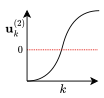
\includegraphics[width=\textwidth]{images/spec_u.png}
    %     % \caption{}
    %     \label{fig:spec_1}
    % \end{subfigure}
    % \hfill
    % \begin{subfigure}[b]{0.23\textwidth}
    %     \centering
    %     \includegraphics[width=\textwidth]{images/spec_g.drawio.png}
    %     % \caption{}
    %     \label{fig:spec_2}
    % \end{subfigure}
    \includegraphics[width=.5\textwidth]{images/spec_u_g.png}
    \caption{
    Visualizing the sorted Fiedler values $\mathbf{u}^{(2)}_1 < \mathbf{u}^{(2)}_2 < \dots < \mathbf{u}^{(2)}_n$, where each entry $\mathbf{u}^{(2)}_i$ corresponds to the vertex assigned to position
    $i$ in the ordering (left), and their mapping to the resulting graph partition (right) obtained by thresholding $\mathbf{u}^{(2)}$ at a value $\epsilon$, set to $0$ or the median.
    }
    \label{fig:spec}
\end{figure}